The rising of quantum computing in the last few year became the attention of researchers to schemes that uses cryptography primitives different from discrete logarithm and number factorization. As mentioned before in Chapter \ref{ch:intro}, code-based cryptosystems are those who uses fundamental aspects of coding theory to add redundancy to a plain text, to intentionally add errors and recovery the plain text. 

In this Chapter, we will explain the first cryptosystem based on coding theory. Furthermore, we will show an Round One code-based submission to the NIST standardization process, the BIGQUAKE, and we show the timing side-channel attack performed in the reference implementation of the scheme.

\section{McEliece Cryptosystem}
Robert J. McEliece proposes in 1978 the first cryptosystem based on coding theory, the McEliece cryptosystem was based on the Goppa codes and uses them to achieve three main algorithms, i. e. Key Generation, Encryption and Decryption \cite{mceliece1978public}. The Figure \ref{fig:code-idea} shows the main of the McEliece Cryptosystem and most of schemes based in coding theory. 

% \begin{figure}[t]
%   \centering
%   \caption{Logotipo da Universidade Federal de Santa Catarina.}
%   \label{fig:logo}

%   \includegraphics[width=.2\linewidth]{../logo-ufsc.pdf}
%   \fonte{o autor.}
% \end{figure}

\begin{figure}
    \centering
    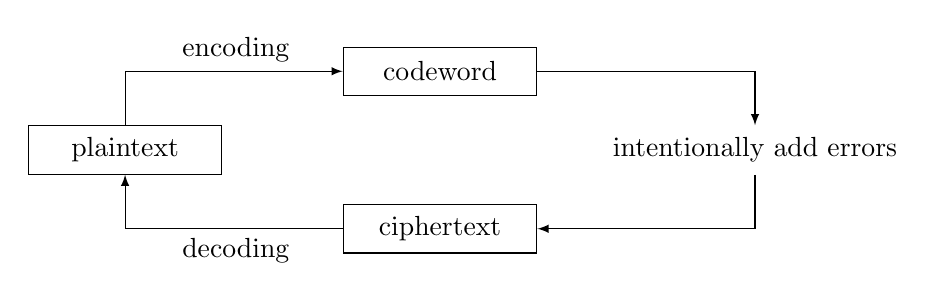
\begin{tikzpicture}
    \node[draw, minimum width=70pt, minimum height=17.5pt] (plain1) at (0, -1) {plaintext};
    \node[draw, minimum width=70pt, minimum height=17.5pt] (ciphertext) at (4, -2) {ciphertext};
    \node[draw, minimum width=70pt, minimum height=17.5pt] (codeword) at (4, 0) {codeword};
    \node[minimum width=70pt, minimum height=17.5pt] (adderror) at (8, -1) {intentionally add errors};
    \draw[-latex] (plain1) |- node[above, xshift=40pt]{encoding} (codeword);
    \draw[-latex] (codeword) -| (adderror);
    \draw[-latex] (adderror) |- (ciphertext);
    \draw[-latex] (ciphertext) -| node[below, xshift=40pt]{decoding} (plain1);
    \end{tikzpicture}
    \label{fig:code-idea}
    \fonte{the author.}
    \caption{Logotipo da Universidade Federal de Santa Catarina.}
\end{figure}

\subsection{Definitions}
\subsection{Decryption}
\section{BIGQUAKE}
\subsection{Submission overview}
\subsection{Timing side-channel attack}